% Created by tikzDevice version 0.12.3.1 on 2023-06-16 15:03:29
% !TEX encoding = UTF-8 Unicode
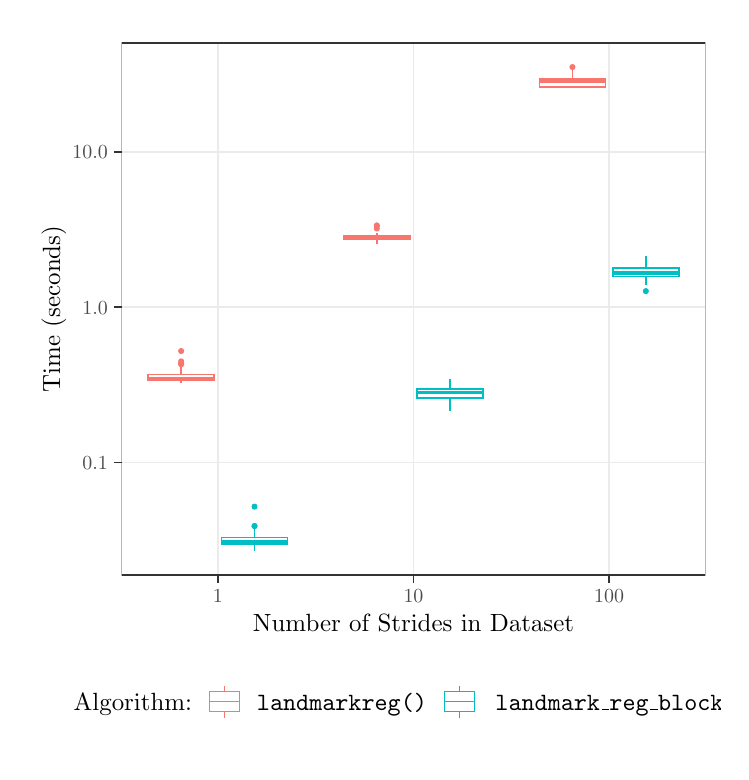
\begin{tikzpicture}[x=1pt,y=1pt]
\definecolor{fillColor}{RGB}{255,255,255}
\path[use as bounding box,fill=fillColor,fill opacity=0.00] (0,0) rectangle (250.38,261.76);
\begin{scope}
\path[clip] (  0.00,  0.00) rectangle (250.38,261.76);
\definecolor{drawColor}{RGB}{255,255,255}
\definecolor{fillColor}{RGB}{255,255,255}

\path[draw=drawColor,line width= 0.6pt,line join=round,line cap=round,fill=fillColor] (  0.00, -0.00) rectangle (250.38,261.76);
\end{scope}
\begin{scope}
\path[clip] ( 33.94, 63.96) rectangle (244.88,256.26);
\definecolor{fillColor}{RGB}{255,255,255}

\path[fill=fillColor] ( 33.94, 63.96) rectangle (244.88,256.26);
\definecolor{drawColor}{gray}{0.92}

\path[draw=drawColor,line width= 0.6pt,line join=round] ( 33.94,104.62) --
	(244.88,104.62);

\path[draw=drawColor,line width= 0.6pt,line join=round] ( 33.94,160.75) --
	(244.88,160.75);

\path[draw=drawColor,line width= 0.6pt,line join=round] ( 33.94,216.89) --
	(244.88,216.89);

\path[draw=drawColor,line width= 0.6pt,line join=round] ( 68.72, 63.96) --
	( 68.72,256.26);

\path[draw=drawColor,line width= 0.6pt,line join=round] (139.41, 63.96) --
	(139.41,256.26);

\path[draw=drawColor,line width= 0.6pt,line join=round] (210.11, 63.96) --
	(210.11,256.26);
\definecolor{drawColor}{RGB}{248,118,109}
\definecolor{fillColor}{RGB}{248,118,109}

\path[draw=drawColor,line width= 0.4pt,line join=round,line cap=round,fill=fillColor] ( 55.46,144.91) circle (  0.89);

\path[draw=drawColor,line width= 0.4pt,line join=round,line cap=round,fill=fillColor] ( 55.46,140.41) circle (  0.89);

\path[draw=drawColor,line width= 0.4pt,line join=round,line cap=round,fill=fillColor] ( 55.46,140.12) circle (  0.89);

\path[draw=drawColor,line width= 0.4pt,line join=round,line cap=round,fill=fillColor] ( 55.46,141.18) circle (  0.89);

\path[draw=drawColor,line width= 0.6pt,line join=round] ( 55.46,136.43) -- ( 55.46,139.26);

\path[draw=drawColor,line width= 0.6pt,line join=round] ( 55.46,134.38) -- ( 55.46,133.43);
\definecolor{fillColor}{RGB}{255,255,255}

\path[draw=drawColor,line width= 0.6pt,fill=fillColor] ( 43.53,136.43) --
	( 43.53,134.38) --
	( 67.39,134.38) --
	( 67.39,136.43) --
	( 43.53,136.43) --
	cycle;

\path[draw=drawColor,line width= 1.1pt] ( 43.53,135.06) -- ( 67.39,135.06);
\definecolor{fillColor}{RGB}{248,118,109}

\path[draw=drawColor,line width= 0.4pt,line join=round,line cap=round,fill=fillColor] (126.16,190.31) circle (  0.89);

\path[draw=drawColor,line width= 0.4pt,line join=round,line cap=round,fill=fillColor] (126.16,189.19) circle (  0.89);

\path[draw=drawColor,line width= 0.4pt,line join=round,line cap=round,fill=fillColor] (126.16,190.11) circle (  0.89);

\path[draw=drawColor,line width= 0.6pt,line join=round] (126.16,186.36) -- (126.16,187.54);

\path[draw=drawColor,line width= 0.6pt,line join=round] (126.16,185.22) -- (126.16,183.76);
\definecolor{fillColor}{RGB}{255,255,255}

\path[draw=drawColor,line width= 0.6pt,fill=fillColor] (114.23,186.36) --
	(114.23,185.22) --
	(138.09,185.22) --
	(138.09,186.36) --
	(114.23,186.36) --
	cycle;

\path[draw=drawColor,line width= 1.1pt] (114.23,185.96) -- (138.09,185.96);
\definecolor{fillColor}{RGB}{248,118,109}

\path[draw=drawColor,line width= 0.4pt,line join=round,line cap=round,fill=fillColor] (196.85,247.52) circle (  0.89);

\path[draw=drawColor,line width= 0.6pt,line join=round] (196.85,243.12) -- (196.85,246.36);

\path[draw=drawColor,line width= 0.6pt,line join=round] (196.85,240.32) -- (196.85,239.85);
\definecolor{fillColor}{RGB}{255,255,255}

\path[draw=drawColor,line width= 0.6pt,fill=fillColor] (184.92,243.12) --
	(184.92,240.32) --
	(208.78,240.32) --
	(208.78,243.12) --
	(184.92,243.12) --
	cycle;

\path[draw=drawColor,line width= 1.1pt] (184.92,242.22) -- (208.78,242.22);
\definecolor{drawColor}{RGB}{0,191,196}
\definecolor{fillColor}{RGB}{0,191,196}

\path[draw=drawColor,line width= 0.4pt,line join=round,line cap=round,fill=fillColor] ( 81.97, 88.68) circle (  0.89);

\path[draw=drawColor,line width= 0.4pt,line join=round,line cap=round,fill=fillColor] ( 81.97, 81.67) circle (  0.89);

\path[draw=drawColor,line width= 0.4pt,line join=round,line cap=round,fill=fillColor] ( 81.97, 81.67) circle (  0.89);

\path[draw=drawColor,line width= 0.6pt,line join=round] ( 81.97, 77.59) -- ( 81.97, 81.03);

\path[draw=drawColor,line width= 0.6pt,line join=round] ( 81.97, 75.27) -- ( 81.97, 72.70);
\definecolor{fillColor}{RGB}{255,255,255}

\path[draw=drawColor,line width= 0.6pt,fill=fillColor] ( 70.04, 77.59) --
	( 70.04, 75.27) --
	( 93.90, 75.27) --
	( 93.90, 77.59) --
	( 70.04, 77.59) --
	cycle;

\path[draw=drawColor,line width= 1.1pt] ( 70.04, 76.07) -- ( 93.90, 76.07);

\path[draw=drawColor,line width= 0.6pt,line join=round] (152.67,131.20) -- (152.67,134.88);

\path[draw=drawColor,line width= 0.6pt,line join=round] (152.67,127.96) -- (152.67,123.17);

\path[draw=drawColor,line width= 0.6pt,fill=fillColor] (140.74,131.20) --
	(140.74,127.96) --
	(164.60,127.96) --
	(164.60,131.20) --
	(140.74,131.20) --
	cycle;

\path[draw=drawColor,line width= 1.1pt] (140.74,129.77) -- (164.60,129.77);
\definecolor{fillColor}{RGB}{0,191,196}

\path[draw=drawColor,line width= 0.4pt,line join=round,line cap=round,fill=fillColor] (223.37,166.56) circle (  0.89);

\path[draw=drawColor,line width= 0.6pt,line join=round] (223.37,174.93) -- (223.37,179.13);

\path[draw=drawColor,line width= 0.6pt,line join=round] (223.37,171.80) -- (223.37,168.64);
\definecolor{fillColor}{RGB}{255,255,255}

\path[draw=drawColor,line width= 0.6pt,fill=fillColor] (211.44,174.93) --
	(211.44,171.80) --
	(235.30,171.80) --
	(235.30,174.93) --
	(211.44,174.93) --
	cycle;

\path[draw=drawColor,line width= 1.1pt] (211.44,173.11) -- (235.30,173.11);
\definecolor{drawColor}{gray}{0.20}

\path[draw=drawColor,line width= 0.6pt,line join=round,line cap=round] ( 33.94, 63.96) rectangle (244.88,256.26);
\end{scope}
\begin{scope}
\path[clip] (  0.00,  0.00) rectangle (250.38,261.76);
\definecolor{drawColor}{gray}{0.30}

\node[text=drawColor,anchor=base east,inner sep=0pt, outer sep=0pt, scale=  0.72] at ( 28.99,102.14) {0.1};

\node[text=drawColor,anchor=base east,inner sep=0pt, outer sep=0pt, scale=  0.72] at ( 28.99,158.28) {1.0};

\node[text=drawColor,anchor=base east,inner sep=0pt, outer sep=0pt, scale=  0.72] at ( 28.99,214.41) {10.0};
\end{scope}
\begin{scope}
\path[clip] (  0.00,  0.00) rectangle (250.38,261.76);
\definecolor{drawColor}{gray}{0.20}

\path[draw=drawColor,line width= 0.6pt,line join=round] ( 31.19,104.62) --
	( 33.94,104.62);

\path[draw=drawColor,line width= 0.6pt,line join=round] ( 31.19,160.75) --
	( 33.94,160.75);

\path[draw=drawColor,line width= 0.6pt,line join=round] ( 31.19,216.89) --
	( 33.94,216.89);
\end{scope}
\begin{scope}
\path[clip] (  0.00,  0.00) rectangle (250.38,261.76);
\definecolor{drawColor}{gray}{0.20}

\path[draw=drawColor,line width= 0.6pt,line join=round] ( 68.72, 61.21) --
	( 68.72, 63.96);

\path[draw=drawColor,line width= 0.6pt,line join=round] (139.41, 61.21) --
	(139.41, 63.96);

\path[draw=drawColor,line width= 0.6pt,line join=round] (210.11, 61.21) --
	(210.11, 63.96);
\end{scope}
\begin{scope}
\path[clip] (  0.00,  0.00) rectangle (250.38,261.76);
\definecolor{drawColor}{gray}{0.30}

\node[text=drawColor,anchor=base,inner sep=0pt, outer sep=0pt, scale=  0.72] at ( 68.72, 54.05) {1};

\node[text=drawColor,anchor=base,inner sep=0pt, outer sep=0pt, scale=  0.72] at (139.41, 54.05) {10};

\node[text=drawColor,anchor=base,inner sep=0pt, outer sep=0pt, scale=  0.72] at (210.11, 54.05) {100};
\end{scope}
\begin{scope}
\path[clip] (  0.00,  0.00) rectangle (250.38,261.76);
\definecolor{drawColor}{RGB}{0,0,0}

\node[text=drawColor,anchor=base,inner sep=0pt, outer sep=0pt, scale=  0.90] at (139.41, 43.70) {Number of Strides in Dataset};
\end{scope}
\begin{scope}
\path[clip] (  0.00,  0.00) rectangle (250.38,261.76);
\definecolor{drawColor}{RGB}{0,0,0}

\node[text=drawColor,rotate= 90.00,anchor=base,inner sep=0pt, outer sep=0pt, scale=  0.90] at ( 11.70,160.11) {Time (seconds)};
\end{scope}
\begin{scope}
\path[clip] (  0.00,  0.00) rectangle (250.38,261.76);
\definecolor{fillColor}{RGB}{255,255,255}

\path[fill=fillColor] ( 11.14,  5.50) rectangle (267.69, 30.95);
\end{scope}
\begin{scope}
\path[clip] (  0.00,  0.00) rectangle (250.38,261.76);
\definecolor{drawColor}{RGB}{0,0,0}

\node[text=drawColor,anchor=base west,inner sep=0pt, outer sep=0pt, scale=  0.90] at ( 16.64, 15.13) {Algorithm:};
\end{scope}
\begin{scope}
\path[clip] (  0.00,  0.00) rectangle (250.38,261.76);
\definecolor{fillColor}{RGB}{255,255,255}

\path[fill=fillColor] ( 63.90, 11.00) rectangle ( 78.35, 25.45);
\end{scope}
\begin{scope}
\path[clip] (  0.00,  0.00) rectangle (250.38,261.76);
\definecolor{drawColor}{RGB}{248,118,109}

\path[draw=drawColor,line width= 0.6pt] ( 71.13, 12.45) --
	( 71.13, 14.61);

\path[draw=drawColor,line width= 0.6pt] ( 71.13, 21.84) --
	( 71.13, 24.01);
\definecolor{fillColor}{RGB}{255,255,255}

\path[draw=drawColor,line width= 0.6pt,fill=fillColor] ( 65.71, 14.61) rectangle ( 76.55, 21.84);

\path[draw=drawColor,line width= 0.6pt] ( 65.71, 18.23) --
	( 76.55, 18.23);
\end{scope}
\begin{scope}
\path[clip] (  0.00,  0.00) rectangle (250.38,261.76);
\definecolor{fillColor}{RGB}{255,255,255}

\path[fill=fillColor] (148.76, 11.00) rectangle (163.22, 25.45);
\end{scope}
\begin{scope}
\path[clip] (  0.00,  0.00) rectangle (250.38,261.76);
\definecolor{drawColor}{RGB}{0,191,196}

\path[draw=drawColor,line width= 0.6pt] (155.99, 12.45) --
	(155.99, 14.61);

\path[draw=drawColor,line width= 0.6pt] (155.99, 21.84) --
	(155.99, 24.01);
\definecolor{fillColor}{RGB}{255,255,255}

\path[draw=drawColor,line width= 0.6pt,fill=fillColor] (150.57, 14.61) rectangle (161.41, 21.84);

\path[draw=drawColor,line width= 0.6pt] (150.57, 18.23) --
	(161.41, 18.23);
\end{scope}
\begin{scope}
\path[clip] (  0.00,  0.00) rectangle (250.38,261.76);
\definecolor{drawColor}{RGB}{0,0,0}

\node[text=drawColor,anchor=base,inner sep=0pt, outer sep=0pt, scale=  0.90] at (113.56, 15.13) {\texttt{landmarkreg()}};
\end{scope}
\begin{scope}
\path[clip] (  0.00,  0.00) rectangle (250.38,261.76);
\definecolor{drawColor}{RGB}{0,0,0}

\node[text=drawColor,anchor=base,inner sep=0pt, outer sep=0pt, scale=  0.90] at (214.96, 15.13) {\texttt{landmark\_reg\_block()}};
\end{scope}
\end{tikzpicture}
